\documentclass[15pt]{beamer}
%
% Choose how your presentation looks.
%
% For more themes, color themes and font themes, see:
% http://deic.uab.es/~iblanes/beamer_gallery/index_by_theme.html
%
\mode<presentation>

{
  \usetheme{PaloAlto}      % or try Darmstadt, Madrid, Warsaw, ...
  \usecolortheme{whale} % or try albatross, beaver, crane, ...
  \usefonttheme{default}  % or try serif, structurebold, ...
  \setbeamertemplate{navigation symbols}{}
  \setbeamertemplate{caption}[numbered]
} 
%remove navigation symbols at bottom
\setbeamertemplate{navigation symbols}{}
\setbeamertemplate{footline}[frame number]
\setbeamertemplate{footline}[text line] {

	\makebox[.7\paperwidth]{
		\insertframenumber  /\inserttotalframenumber
		\hfill
		\url{http://envirohack.herokuapp.com/}
	}

}

% add logo
\usepackage{pgf}
%coords are in relation to lower right corner
\logo{\pgfputat{\pgfxy(-1,8)}{\pgfbox[center,base]{\includegraphics[width=1.7cm]{logo.jpg}}}}


%I had problems compiling doc on X230 without next two lines
\usepackage{etex}
\reserveinserts{28}
%On X530 it worked without problems

%\usepackage[utf8x]{inputenc}
\input{Preamble.tex}
%\renewcommand{\baselinestretch}{1.2} %line spacing
%{\setstretch{1.0}\color{blue} text bla bla } for section strech
\renewcommand{\footnotesize}{\scriptsize}
%\usepackage[demo]{graphicx}
\usepackage{caption}
%\usepackage{subcaption}

\title[EnviroHack]{Maximise your energy usage with our daily energy forecast}
\author{Energy Cast}
%\institute{eCast}
%\date{25/01/2015}

\begin{document}
	


%\begin{frame}
%	\titlepage
%\end{frame}

%[plain] so we get no logo on this page
\begin{frame}[plain]{}
	\begin{figure}
		
		
\includegraphics[width=0.9\textwidth]{pic/energycast-splash.pdf}
		%\caption{intro}
	\end{figure}	
\url{http://envirohack.herokuapp.com/}
\end{frame}

% Uncomment these lines for an automatically generated outline.
%\begin{frame}{Outline}
%  \tableofcontents
%\end{frame}

\section{Define problem}

\begin{frame}{Solar panels}
	\begin{itemize}
		
		\item Cut your carbon footprint.
		\item Cut your electricity bills.
		\item Get paid for the electricity you generate. 

	\end{itemize}
	

\end{frame}

\section{Market research}

\begin{frame}{We use more green power}
	\begin{table}
		\centering
		\begin{minipage}[t]{\textwidth}%
			\resizebox{\columnwidth}{!}{%
				\begin{tabular}{lcccccc} %{l|c|c|c|c}
					\toprule %\rowcolor{lightgray}
					&2000 & 2009 & 2010 & 2011 & 2012 & 2013\tabularnewline
					\midrule
					Nuclear & 8.4\% & 7.2\% & 6.4\% & 7.7\% & 7.3\% & 7.5\%\\
					Wind & 0.0\% & 0.4\% & 0.4\% & 0.7\% & 0.8\% & 1.2\%\\
					Hydro & 0.2\% & 0.2\% & 0.1\% & 0.2\% & 0.2\% & 0.2\%\\
					Bioenergy & 0.9\% & 2.1\% & 2.3\% & 2.6\% & 2.8\% & 3.3\%\\
					Transport fuels & 0.0\% & 0.5\% & 0.6\% & 0.6\% & 0.5\% & 0.5\%\\
					Other & 0.0\% & 0.0\% & 0.1\% & 0.1\% & 0.2\% & 0.2\%\\
					\midrule
					\textbf{Total} & 9.4\% & 104.\% & 9.8\% & 11.9\% & 11.8\% & 12.9\%\\
					\bottomrule
				\end{tabular}%
			}
			\caption{Low carbon energy sources}
		\end{minipage}
	\end{table}

\end{frame}

\begin{frame}{And a lot of solar panels}
	\begin{table}
		\centering
		\begin{minipage}[t]{\textwidth}%
			\resizebox{\columnwidth}{!}{%
				\begin{tabular}{lcccc} %{l|c|c|c|c}
					\toprule %\rowcolor{lightgray}
					type & 2011 Q1 & 2012 Q1 & 2013 Q1 & 2014 Q1\\
					\midrule
					Micro CHP & 0.1 & 0.4 & 0.5 & 0.5\\
					Anaerobic Digestion & 1.8 & 14 & 38 & 68\\
					Hydro & 10 & 22 & 35 & 46\\
					Wind & 18 & 54 & 133 & 215\\
					Solar & 77 & 998 & 1,583 & 2,056\\
					\bottomrule
				\end{tabular}%
			}
			\caption{Cumulative Installed capacity (MW)}
		\end{minipage}
	\end{table}
\end{frame}

\section{Details}
	\begin{frame}
	\begin{figure}
		\centering
		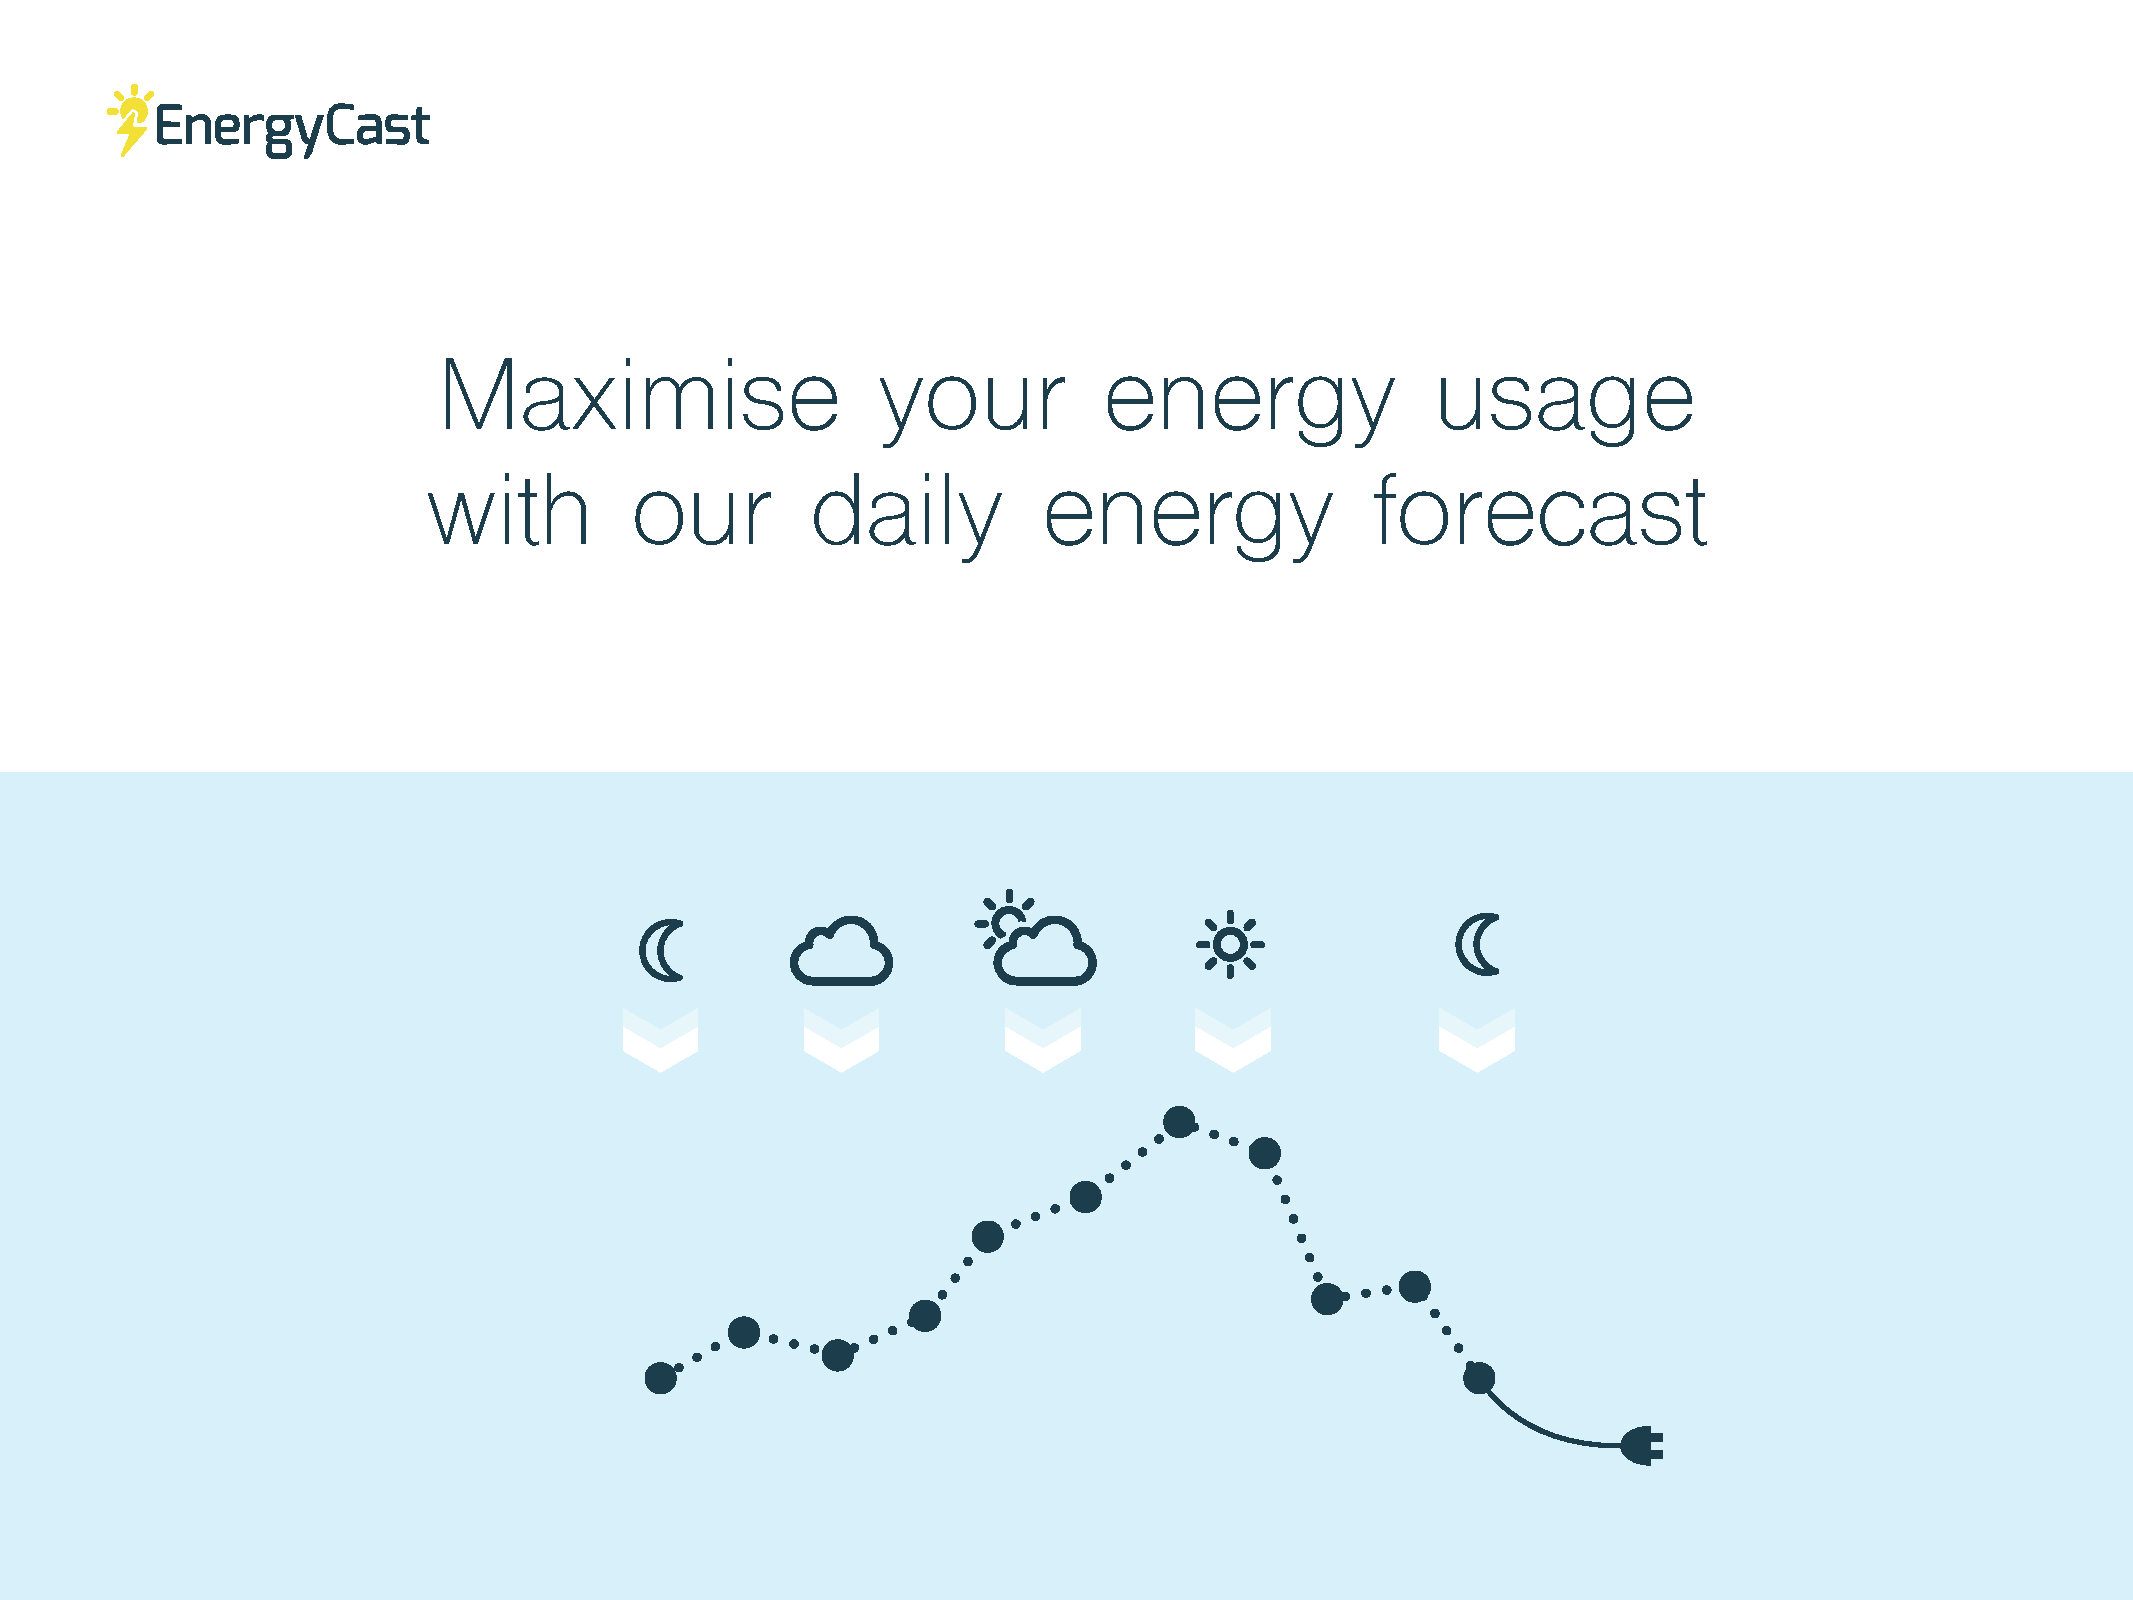
\includegraphics[height=0.8\textheight]{pic/energycast-gaphic.pdf}
		%\caption{Locust attack}
	\end{figure}	
	\end{frame}

\begin{frame}{System overview}
	
	\begin{figure} %this is tikZ figure! dont include .tex
		%	\centering
		%	\includestandalone[height=.8\textheight]{pic/SoftwareWorkflow}
		\includegraphics[width=0.7\textwidth]{pic/SoftwareWorkflow.pdf}
		
		%\caption{System overview}
	\end{figure}
	
	\url{http://envirohack.herokuapp.com/}
\end{frame}

\begin{frame}{Unlocking data}
	\begin{figure}
		\centering
		\includegraphics[width=1.0\textwidth]{pic/dataPoint.jpg}
		%\caption{Locust attack}
	\end{figure}

\end{frame}

\begin{frame}{Machine Learning}
	\begin{figure}
		\centering
		\includegraphics[width=1.0\textwidth]{pic/MLmodel.png}
		%\caption{Locust attack}
	\end{figure}
	
	\url{http://envirohack.herokuapp.com/}
\end{frame}

\begin{frame}{Machine Learning model accuracy}
	\begin{figure}
		%\centering
		\includegraphics[height=0.9\textheight]{pic/MLaccuracy.png}
		%\caption{Locust attack}
	\end{figure}

\end{frame}


\begin{frame}{Taking things forward}
\begin{Large} %make text large
	\begin{itemize}
		\item Smart information
		\item  Smart decisions
		\item Smart devices
	\end{itemize}
\end{Large}
\end{frame}

\end{document}
